\documentclass[12pt]{article}
\usepackage[left=1cm, right=1cm, top=2cm,bottom=1.5cm]{geometry} 

\usepackage[parfill]{parskip}
\usepackage[utf8]{inputenc}
\usepackage[T2A]{fontenc}
\usepackage[russian]{babel}
\usepackage{enumitem}
\usepackage[normalem]{ulem}
\usepackage{amsfonts, amsmath, amsthm, amssymb, mathtools}

\usepackage{accents}
\usepackage{fancyhdr}
\pagestyle{fancy}
\renewcommand{\headrulewidth}{1.5pt}
\renewcommand{\footrulewidth}{1pt}

\usepackage{graphicx}
\usepackage[figurename=Рис.]{caption}
\usepackage{subcaption}
\usepackage{float}

%%Наименование папки откуда забирать изображения
\graphicspath{ {./images/} }

%%Изменение формата для ввода доказательства
\renewcommand{\proofname}{$\square$  \nopunct}
\renewcommand\qedsymbol{$\blacksquare$}

\addto\captionsrussian{%
	\renewcommand{\proofname}{$\square$ \nopunct}%
}
%% Римские цифры
\newcommand{\RN}[1]{%
	\textup{\uppercase\expandafter{\romannumeral#1}}%
}

%% Для удобства записи
\newcommand{\MR}{\mathbb{R}}
\newcommand{\MQ}{\mathbb{Q}}
\newcommand{\MI}{\mathrm{I}}
\newcommand{\MJ}{\mathrm{J}}
\newcommand{\MH}{\mathrm{H}}
\newcommand{\MT}{\mathrm{T}}
\newcommand{\MU}{\mathcal{U}}
\newcommand{\MV}{\mathcal{V}}
\newcommand{\VN}{\varnothing}
\newcommand{\VE}{\varepsilon}

\theoremstyle{definition}
\newtheorem{defn}{Опр:}
\newtheorem{rem}{Rm:}
\newtheorem{prop}{Утв.}
\newtheorem{exrc}{Упр.}
\newtheorem{lemma}{Лемма}
\newtheorem{theorem}{Теорема}
\newtheorem{corollary}{Следствие}

\newenvironment{cusdefn}[1]
{\renewcommand\thedefn{#1}\defn}
{\enddefn}

\DeclareRobustCommand{\divby}{%
	\mathrel{\text{\vbox{\baselineskip.65ex\lineskiplimit0pt\hbox{.}\hbox{.}\hbox{.}}}}%
}
%Короткий минус
\DeclareMathSymbol{\SMN}{\mathbin}{AMSa}{"39}

%Функция знака
\DeclareMathOperator{\sgn}{sgn}

\newcommand{\smallerrel}[1]{\mathrel{\mathpalette\smallerrelaux{#1}}}
\newcommand{\smallerrelaux}[2]{\raisebox{.1ex}{\scalebox{.75}{$#1#2$}}}

\newcommand{\smallin}{\smallerrel{\in}}
\newcommand{\smallnotin}{\smallerrel{\notin}}

\newcommand*{\medcap}{\mathbin{\scalebox{1.25}{\ensuremath{\cap}}}}%
\newcommand*{\medcup}{\mathbin{\scalebox{1.25}{\ensuremath{\cup}}}}%

%Подпись символов снизу
\newcommand{\ubar}[1]{\underaccent{\bar}{#1}}

\begin{document}
\lhead{Математический анализ - I}
\chead{Шапошников С.В.}
\rhead{Лекция - 28}
\section*{Выпуклость функций}
	
\begin{defn}
	$f$ \uwave{выпукла на $(a,b)$}, если $\forall x, y \in (a,b) \wedge \forall \alpha \in [0,1], \, f(\alpha x + (1-\alpha) y) \leq \alpha f(x) + (1-\alpha)f(y)$.
\end{defn}
\begin{rem}
	Геометрически выпуклость $\Leftrightarrow$ любая хорда лежит выше графика $\Leftrightarrow$ тангенсы углов наклона хорд не убывают, если их располагать вдоль графика.
\end{rem}

\begin{theorem}
	Пусть $f$ - дифференцируема на интервале $(a,b)$, тогда следующие утверждения эквивалентны:
	\begin{enumerate}[label={(\arabic*)}]
		\item $f$ - выпукла на $(a,b)$;
		\item $f^\prime$ - не убывает на $(a,b)$;
		\item $f(x) \geq f(y) + f^\prime(y)(x-y), \, \forall x,y, \in (a,b)$;
	\end{enumerate}
\end{theorem}
\begin{proof}\hfill\\
	$(3) \Rightarrow (1)$: Возьмем точки $x_1,x,x_2 \in (a,b) \colon x_1 < x < x_2$. Докажем, что $\dfrac{f(x) - f(x_1)}{x - x_1} \leq \dfrac{f(x_2) - f(x)}{x_2 - x}$.
	\begin{figure}[H]
		\centering
		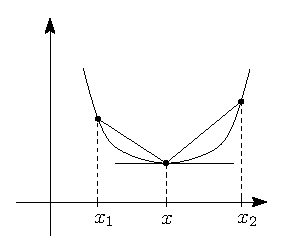
\includegraphics[width=0.3\textwidth]{28_1.eps}
		\caption{Сравнение наклона хорд с наклоном касательной в точке $x$.}
		\label{28_1}
	\end{figure}
	Рассмотрим точки $x$ и $x_1 \Rightarrow$ по условию $f(x_1) \geq f(x) + f^\prime(x)(x_1 - x) \Rightarrow f^\prime(x)(x - x_1) \geq f(x) - f(x_1) \Rightarrow$\\
	$\Rightarrow$ поскольку $x > x_1 \Rightarrow f^\prime(x) \geq \dfrac{f(x) - f(x_1)}{x - x_1}$.
	
	Рассмотрим точки $x_2$ и $x \Rightarrow$ по условию $f(x_2) \geq f(x) + f^\prime(x)(x_2 - x) \Rightarrow f(x_2) - f(x) \geq f^\prime(x)(x_2 - x) \Rightarrow$\\
	$\Rightarrow$ поскольку $x_2 > x \Rightarrow \dfrac{f(x_2) - f(x)}{x_2 - x} \geq f^\prime(x)$.	
	
	Таким образом мы получаем, что $\dfrac{f(x) - f(x_1)}{x - x_1} \leq f^\prime(x) \leq \dfrac{f(x_2) - f(x)}{x_2 - x}$.
\end{proof}

\begin{corollary}
	Пусть $f$ дважды дифференцируема на интервале $(a,b)$. Тогда $f$ - выпукла $\Leftrightarrow f^{\prime\prime} \geq 0$.
\end{corollary}

\begin{proof}
	$f^\prime$ - не убывает $\Leftrightarrow f^{\prime\prime} \geq 0$.
\end{proof}
\newpage
\subsection*{Неравенство Йенсена}
\begin{theorem}\textbf{(Неравенство Йенсена)}
	Пусть $f$ выпукла на $(a,b)$, $\alpha_1, \dotsc, \alpha_n \in [0,1]\colon \displaystyle \sum\limits_{k=1}^{n}\alpha_k = 1$,\\
	$x_1, \dotsc , x_n \in (a,b)$, тогда $f(\alpha_1 x_1 + \dotsc + \alpha_n x_n) \leq \alpha_1 f(x_1) + \dotsc + \alpha_n f(x_n)$.
\end{theorem}
\begin{proof}
	Индукцией по $n$ (все $\alpha_i \geq 0$):\\
	\uline{База}: $n = 1 \Rightarrow \alpha_1 = 1, \, f(x_1) \leq f(x_1)$; $n = 2 \Rightarrow \alpha_1 + \alpha_2 = 1, \, f(\alpha_1 x_1 + \alpha_2 x_2) \leq \alpha_1 f(x_1) + \alpha_2 f(x_2)$ - по определению выпуклости.\\
	\uline{Шаг}: Пусть $S_n = \displaystyle \sum\limits_{k=1}^{n}\alpha_k$ и утверждение доказано для $n$, докажем для $n+1$ (случай, когда $\alpha_1 = \dotsc = \alpha_n = 0, \, \alpha_{n+1} = 1$ очевиден):
	$$f(\alpha_1 x_1 + \dotsc + \alpha_n x_n + \alpha_{n+1} x_{n+1}) = f\Big((\alpha_1 + \dotsc + \alpha_n)\Big(\dfrac{\alpha_1}{S_n}x_1 + \dotsc + \dfrac{\alpha_n}{S_n}x_n\Big) + \alpha_{n+1} x_{n+1}\Big)$$
	Из-за выпуклости $f$ и $\displaystyle \sum\limits_{k=1}^{n+1}\alpha_k = S_n + \alpha_{n+1} = 1$ получим:
	$$f(\alpha_1 x_1 + \dotsc + \alpha_{n+1} x_{n+1}) = f\Big(S_n\Big(\dfrac{\alpha_1}{S_n}x_1 + \dotsc + \dfrac{\alpha_n}{S_n}x_n\Big) + \alpha_{n+1} x_{n+1}\Big) \leq S_nf\Big(\dfrac{\alpha_1}{S_n}x_1 + \dotsc + \dfrac{\alpha_n}{S_n}x_n\Big) + \alpha_{n+1} f(x_{n+1})$$
	где $\beta_1 = \dfrac{\alpha_1}{\alpha_1 + \dotsc + \alpha_n} \geq 0, \dotsc , \beta_ n = \dfrac{\alpha_n}{\alpha_1 + \dotsc + \alpha_n} \geq 0, \, \displaystyle \sum\limits_{k=1}^{n}\beta_n = 1 \Rightarrow$ воспользуемся предположением индукции:
	$$S_nf\Big(\dfrac{\alpha_1}{S_n}x_1 + \dotsc + \dfrac{\alpha_n}{S_n}x_n\Big) + \alpha_{n+1} f(x_{n+1}) \leq  S_n \Big(\beta_1 f(x_1) + \dotsc + \beta_n f(x_n) \Big) + \alpha_{n+1}f(x_{n+1}) = $$
	$$ = S_n{\cdot}\dfrac{\alpha_1}{S_n}f(x_1) + \dotsc + S_n{\cdot}\dfrac{\alpha_n}{S_n}f(x_n) + \alpha_{n+1} f(x_{n+1}) = \alpha_1 f(x_1) + \dotsc + \alpha_{n+1}f(x_{n+1})$$
\end{proof}

\textbf{Пример (ср. арифм-ое $\geq$ ср. геом-ое)}: Пусть $x_i > 0 \Rightarrow \dfrac{x_1 + \dotsc + x_n}{n} \geq \sqrt[n]{x_1{\cdot}\dotsc{\cdot}x_n}$.
\begin{proof}
	$$\dfrac{x_1 + \dotsc + x_n}{n} \geq \sqrt[n]{x_1{\cdot}\dotsc{\cdot}x_n} \Leftrightarrow \ln\Big(\dfrac{x_1 + \dotsc + x_n}{n} \Big) \geq \dfrac{\ln(x_1) + \dotsc + \ln(x_n)}{n} \Leftrightarrow$$
	$$\Leftrightarrow  -\ln\Big(\dfrac{x_1 + \dotsc + x_n}{n} \Big) \leq -\dfrac{\ln(x_1)}{n} - \dotsc - \dfrac{\ln(x_n)}{n}$$
	Функция $f(x) = -\ln{x}$ - выпукла: $f^\prime(x) = 	- \dfrac{1}{x}, \, f^{\prime\prime}(x) = \dfrac{1}{x^2} > 0 \Rightarrow$ неравенство выше справедливо по неравенству Йенсена.
\end{proof}

\textbf{Пример (энтропия)}: $f(x) = x\ln{x},\, x > 0$; $f(x)$ - выпукла: $(x\ln{x})^{\prime\prime} = (\ln{x} + 1)^\prime = \dfrac{1}{x} > 0$. Функция энтропии дает характеристику, насколько неопределенна ситуация: когда все варианты равновероятны $\Rightarrow$ это ситуация с минимальной определенностью $\Rightarrow$ максимальная энтропия; когда только один вариант возможен $\Rightarrow$ это ситуация с максимальной определенностью $\Rightarrow$ минимальная энтропия.
\begin{defn}
	Функция \uwave{энтропии}: $H(p) = -\displaystyle \sum\limits_{i = 1}^{n} p_i \ln{p_i}$.
\end{defn}
Если $\forall i =\overline{1,n},\, p_i = \frac{1}{n} \Rightarrow H(p) = -\frac{n}{n}\ln{\frac{1}{n}} = \ln{n}$. 

Предположим, что мы кодируем слова, используя $0$ и $1$, тогда для слов длины $n$ пришлось бы сделать $2^n$ кодов. Длина слова, которое можно закодировать равна $\ln{2^n} = n$. Есть набор слов, спрашивается: какой длины коды будем писать $\Rightarrow$ возникает логарифм.

Сравним функцию $H(p)$ и $\ln{n}$. Что больше? Запишем $-\dfrac{1}{n}\ln{n}$ в следующем виде и применим неравенство Йенсена:
$$
-\dfrac{1}{n}\ln{n} = \Big(\dfrac{p_1 + \dotsc + p_n}{n}\Big)\ln{\Big( \dfrac{p_1 + \dotsc + p_n}{n}\Big)} = f\Big(\dfrac{p_1 + \dotsc + p_n}{n} \Big) \leq \dfrac{1}{n}p_1 \ln{p_1} + \dfrac{1}{n}p_2\ln{p_2} + \dotsc + \dfrac{1}{n}p_n\ln{p_n}
$$
Домножаем на $(-n)$ получим:
$$
- \sum\limits_{i=1}^{n} p_i\ln{p_i} = H(p) = H(\{p_1, \dotsc, p_n \}) \leq \ln{n} = H(\{\tfrac{1}{n},\dotsc,\tfrac{1}{n} \})
$$
Таким образом, энтропия всегда меньше или равна энтропии в самой неопределенной ситуации. 
Энтропия минимальна, когда все слагаемые нулевые: $p_i =0 \vee p_i = 1$, где мы определяем $0{\cdot}\!\ln{0} = 0$. В таком случае, один из исходов - достоверный.

\newpage
\subsection*{Строгая выпуклость}
\begin{defn}
	Функция $f$ на интервале $(a,b)$ называется \uwave{строго выпуклой}, если 
	$$\forall x_1, x_2 \in (a,b), x_1 \neq x_2 \wedge \forall \alpha \in (0,1) \colon f(\alpha x_1 + (1 - \alpha) x_2) < \alpha f(x_1) + (1 - \alpha) f(x_2)$$
\end{defn}

\begin{prop}
	Строгая выпуклость $\Leftrightarrow \forall x_1, x_2, x \in (a,b),\, x_1 < x < x_2, \, \dfrac{f(x) - f(x_1)}{x - x_1} < \dfrac{f(x_2) - f(x)}{x_2 - x}$.
\end{prop}
\begin{proof}
	Аналогичное доказательству для простой выпуклости.
\end{proof}

\begin{theorem}
	Пусть $f$ - дифференцируема на интервале $(a,b)$, тогда следующие утверждения эквивалентны:
	\begin{enumerate}[label={(\arabic*)}]
		\item $f$ - строго выпукла на $(a,b)$;
		\item $f^\prime$ - возрастает на $(a,b)$;
		\item $f(x) > f(y) + f^\prime(y)(x-y), \, \forall x \neq y \in (a,b)$;
	\end{enumerate}
\end{theorem}
\begin{proof}\hfill\\
	$(1) \Leftrightarrow (2)$: Здесь уже не получится доказать по аналогии, поскольку строгие неравенства перейдут в нестрогие. Возьмем две точки $x_1, x_2 \in (a,b), \, x_1 < x_2$. Возьмем любую точку $x \in (x_1,x_2)$. Мы знаем, что $\dfrac{f(x) - f(x_1)}{x - x_1} < \dfrac{f(x_2) - f(x)}{x_2 - x}$. По теореме Лагранжа 
	$$\exists \, c_1 \in (x_1,x) \colon f^\prime(c_1) = \dfrac{f(x) - f(x_1)}{x - x_1} \wedge \exists \, c_2 \in (x,x_2) \colon f^\prime(c_2) = \dfrac{f(x_2) - f(x)}{x_2 - x}$$
	\begin{figure}[H]
		\centering
		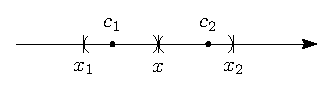
\includegraphics[width=0.35\textwidth]{28_2.eps}
		\caption{Применение теоремы Лагранжа на отрезках $(x_1,x)$ и $(x,x_2)$.}
		\label{28_2}
	\end{figure}
	Поскольку функция выпукла $\Rightarrow$ ее производная не убывает $\Rightarrow f^{\prime}(x_1) \leq f^\prime(c_1) \wedge f^\prime(c_2) \leq f^\prime(x_2)$, тогда:
	$$\forall x_1, x_2 \in (a,b),\, x_1 < x_2, \, f^{\prime}(x_1) \leq f^\prime(c_1) = \dfrac{f(x) - f(x_1)}{x - x_1} < \dfrac{f(x_2) - f(x)}{x_2 - x} = f^{\prime}(c_2) \leq f(x_2)$$
	Доказательство верно и в обратную сторону.
	
	$(2) \Rightarrow (3)$: Рассмотрим несколько случаев:
	\begin{enumerate}[label={\arabic*)}]
		\item Пусть $x > y \Rightarrow$ по теореме Лагранжа: $\exists \, c \in (y,x) \colon \dfrac{f(x) - f(y)}{x - y} = f^\prime(c)$, по пункту $(2)$:
		$$c > y \Rightarrow f^\prime(c) > f^\prime(y) \Rightarrow f(x) - f(y) > f^\prime(y)(x-y) \Rightarrow f(x) > f(y) + f^\prime(y)(x-y)$$
		\item Пусть $y > x \Rightarrow$ по теореме Лагранжа: $\exists \, c \in (x,y) \colon \dfrac{f(y) - f(x)}{y - x} = f^\prime(c)$, по пункту $(2)$:
		$$c < y \Rightarrow f^\prime(c) < f^\prime(y) \Rightarrow f(y) - f(x) < f^\prime(y)(y-x) \Rightarrow f(x) > f(y) + f^\prime(y)(x-y)$$
	\end{enumerate}
	
	$(3) \Rightarrow (1)$: Возьмем точки $x_1,x,x_2 \in (a,b) \colon x_1 < x < x_2$. Докажем, что $\dfrac{f(x) - f(x_1)}{x - x_1} < \dfrac{f(x_2) - f(x)}{x_2 - x}$.

	Рассмотрим точки $x$ и $x_1 \Rightarrow$ по условию $f(x_1) > f(x) + f^\prime(x)(x_1 - x) \Rightarrow f^\prime(x)(x - x_1) > f(x) - f(x_1) \Rightarrow$\\
	$\Rightarrow$ поскольку $x > x_1 \Rightarrow f^\prime(x) > \dfrac{f(x) - f(x_1)}{x - x_1}$.
	
	Рассмотрим точки $x_2$ и $x \Rightarrow$ по условию $f(x_2) > f(x) + f^\prime(x)(x_2 - x) \Rightarrow f(x_2) - f(x) > f^\prime(x)(x_2 - x) \Rightarrow$\\
	$\Rightarrow$ поскольку $x_2 > x \Rightarrow \dfrac{f(x_2) - f(x)}{x_2 - x} > f^\prime(x)$.	
	
	Таким образом мы получаем, что $\dfrac{f(x) - f(x_1)}{x - x_1} < f^\prime(x) < \dfrac{f(x_2) - f(x)}{x_2 - x}$.
\end{proof}

\begin{corollary}
	Пусть $f$ дважды дифференцируема на $(a,b)$. Если $f^{\prime\prime} > 0$, то $f$ строго выпукла.
\end{corollary}

\begin{rem}Необходимо выделить ряд замечаний:
	\begin{enumerate}[label={(\arabic*)}]
		\item Выпуклые функции иногда называют \uwave{выпуклыми вниз} (потому что они провисают);
		\item Если $(-f)$ выпукла, то $f$ называется \uwave{вогнутой функцией} или \uwave{выпуклой вверх};
		\item Если $f$ определена в окрестности $\MU(a)$ и при $x< a, f$ выпукла (вогнута), при $x > a, f$ вогнута (выпукла), то есть $f$ меняет выпуклость в точке $a$, то говорят, что $a$ - \uwave{точка перегиба $f$};
	\end{enumerate}
\end{rem}

\newpage
\section*{Метод касательных или метод Ньютона}
Во многих прикладных задачах, важную роль играет поиск нуля функции: $f(x) = 0$. Способы поиска нуля функции:
\begin{enumerate}[label={\arabic*)}]
	\item \uline{Метод бисекций}: делим пополам и выбираем ту половину на концах которой знаки разные, скорость сходимости к нулю функции $\dfrac{1}{2^n}$;
	\begin{figure}[H]
		\centering
		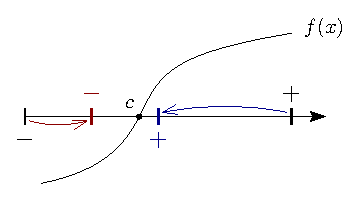
\includegraphics[width=0.35\textwidth]{28_3.eps}
		\caption{Метод бисекций в поиске нуля функции $f(x)$.}
		\label{28_3}
	\end{figure}
	\item \uline{Метод Ньютона}: строим касательные в точках пересечения предыдущей касательной с осью $x$, скорость сходимости к нулю функции $\dfrac{1}{2^{2^n}}$;
\end{enumerate}
\subsection*{Метод Ньютона}
Пусть задана функция $f$ на интервале $(a,b), \, f^\prime(x) \geq \alpha > 0, \, \beta \geq f^{\prime\prime}(x) > 0$ (то есть функция строго монотонна и строго выпукла) и $\exists \, c \in (a,b) \colon f(c) = 0$. Поскольку функция возрастает, то такое $c$ только одно. 

Пусть $x_1 > c$. Будем устраивать последовательность, которая сходится к $c$: 
$$x_n \to x_{n+1} \colon y = f(x_n) + f^\prime(x_n)(x - x_n) \Rightarrow f(x_n) + f^\prime(x_n)(x_{n+1} - x_n) = 0 \Rightarrow x_{n+1} = x_n - \dfrac{ f(x_n)}{f^\prime(x_n)}$$
\begin{figure}[H]
	\centering
	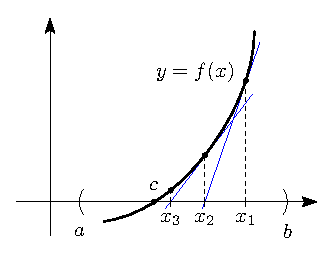
\includegraphics[width=0.4\textwidth]{28_4.eps}
	\caption{Сходимость в методе Ньютона.}
	\label{28_4}
\end{figure}
\newpage
\begin{rem}
	Почему $x_n \to c$?
	\begin{enumerate}[label={(\arabic*)}]
		\item Из-за строгой выпуклости $f(x_{n}) > 0 \Rightarrow$ так как $f(x) > 0$ только справа от $c \Rightarrow  x_{n} > c$;
		\item $x_n$ - убывает: $x_n >c \Rightarrow f(x_n) > 0\wedge f^\prime(x_n) > 0 \Rightarrow \dfrac{f(x_n)}{f^\prime(x_n)}>0 \Rightarrow x_{n+1} = x_n - \dfrac{f(x_n)}{f^\prime(x_n)} < x_n$;
	\end{enumerate}
	Следовательно, $x_n \to a \geq c \Rightarrow $ перейдем к пределу: 
	$$x_{n+1} = x_n - \dfrac{f(x_n)}{f^\prime(x_n)} \Rightarrow a = a - \dfrac{f(a)}{f^\prime(a)} \Rightarrow f(a) = 0 $$ 
	Но у нас есть только одна точка, где $f(x) = 0$ и эта точка $c\Rightarrow a = c$.
\end{rem}

\begin{rem}
	Как быстро эта последовательность стремится к $c$? 
	
	Рассмотрим следующую разность:
	$$|x_{n+1} - c| = \bigg|x_n - \dfrac{f(x_n)}{f^\prime(x_n)} - c\bigg| = \bigg|(x_n - c) - \dfrac{f(x_n)}{f^\prime(x_n)}\bigg|$$
	Применим разложение Тейлора с остаточным членом в форме Лагранжа в точке $x_n$: 
	$$f(t) = f(x_n) + f^\prime(x_n)(t - x_n) + \dfrac{f^{\prime\prime}(u)(t - x_n)^2}{2}$$
	Подставим в разложение $t = c$ : 
	$$0 = f(x_n) + f^\prime(x_n)(c - x_n) + \dfrac{f^{\prime\prime}(u)(c - x_n)^2}{2} \Rightarrow \dfrac{f(x_n)}{f^\prime(x_n)} = - (c-x_n) - \dfrac{f^{\prime\prime}(u)}{2f^\prime(x_n)}(c - x_n)^2 $$
	Подставим это разложение в исходную разность и вспомним, что $f^\prime(x) \geq \alpha > 0 \wedge \beta \geq f^{\prime\prime}(x) > 0$:
	$$ |x_{n+1} - c| = \bigg|\dfrac{f^{\prime\prime}(u)}{2f^\prime(x_n)}(c - x_n)^2\bigg| \leq \dfrac{\beta}{2\alpha}|x_n - c|^2 = M|x_n - c|^2$$
	Таким образом мы получили:
	$$|x_{n+1} - c| \leq M|x_n - c|^2 \leq M^2|x_{n-1} - c|^4 \leq M^{2^{n}}|x_1 - c|^{2^{n}}$$
	Пусть мы изначально выбрали точку так, что $M|x_1 - c| < \dfrac{1}{2} \Rightarrow |x_{n+1} - c| \leq \dfrac{1}{2^{2^n}}$.
\end{rem}
\end{document}